\chapter{Opis projektnog zadatka}
		\textbf{\textit{dio 1. revizije}}\\
		
		\textit{Na osnovi projektnog zadatka detaljno opisati korisničke zahtjeve. Što jasnije opisati cilj projektnog zadatka, razraditi problematiku zadatka, dodati nove aspekte problema i potencijalnih rješenja. Očekuje se minimalno 3, a poželjno 4-5 stranica opisa.	Teme koje treba dodatno razraditi u ovom poglavlju su:}
		\begin{packed_item}
			\item \textit{potencijalna korist ovog projekta}
			\item \textit{postojeća slična rješenja (istražiti i ukratko opisati razlike u odnosu na zadani zadatak). Dodajte slike koja predočavaju slična rješenja.}
			\item \textit{skup korisnika koji bi mogao biti zainteresiran za ostvareno rješenje.}
			\item \textit{mogućnost prilagodbe rješenja }
			\item \textit{opseg projektnog zadatka}
			\item \textit{moguće nadogradnje projektnog zadatka}
		\end{packed_item}
		
		\textit{Za pomoć pogledati reference navedene u poglavlju „Popis literature“, a po potrebi konzultirati sadržaj na internetu koji nudi dobre smjernice u tom pogledu.}
		\eject
		
		Cilj ovog projekta je razviti programsku podršku za stvaranje web aplikacije \textit{Giger} koja je namijenjena glazbenicima, ljudima kojima su potrebne usluge glazbenika (organizatori različitih proslava, menadžeri) te ljudima koji su zainteresirani za obližnje događaje. Na taj način na jednom mjestu se omogućava:
		
		\begin{packed_item}
			\item upoznavanje glazbenika i njihovo povezivanje u bendove
			\item olakšana komunikacija i organizacija unutar bendova
			\item promocija glazbenika
			\item dogovaranje gaža s organizatorima koji jednostavno mogu pronaći prikladan bend za određeni događaj
			\item pregled zanimljivih nadolazećih događaja dostupan svima
			\item uvid u recenzije bendova/organizatora
		\end{packed_item}
	

		Organizacija osobnog kalendara i dogovaranje termina koji zahtijevaju prisustvovanje više ljudi je težak zadatak, a s tim se problemom na gotovo dnevnoj razini susreću glazbenici kada dogovaraju nastupe. Isto tako, ljudi koji organiziraju razne proslave za koje trebaju glazbenike, kao i ljudi koji žele otići na neku živu svirku, ponekad ne znaju kakva je glazbena ponuda u njihovoj okolini, a ako su i čuli za neki događaj u blizini, ne postoji jedinstveno mjesto gdje mogu pročitati recenzije o glazbenicima, bendu ili organizatoru da budu sigurni u kvalitetu događaja.
		\textit{Giger} je platforma koja rješava navedene probleme integrirajući kalendar glazbenika sa servisom namijenjenim za sastajanje bendova i organizatora nastupa. 
		\\
		
		Česta je situacija da je jedan glazbenik član više bendova, pa tako dostupnost svakog benda ovisi o dostupnosti svih njegovih članova.  Kalendar svakog glazbenika ujedinjuje sve obaveze iz bendova u kojima je član pa dostupnost benda postaje trivijalna informacija. 
		
		
		
		\section{Tijek i opseg aplikacije}
		
		Prilikom pokretanja aplikacije, neregistriranom korisniku prikazuju se opće informacije o javnim događajima te mu se nudi mogućnost prijavljivanja u sustav s postojećim računom (potrebno upisati korisničko ime i lozinku) i kreiranje novog računa. Za stvaranje novog računa potrebni su: 
		
		\begin{packed_item}
			\item korisnično ime
			\item email adresa
			\item lozinka
		\end{packed_item}
	
		Registrirani korisnik može pregledati, mijenjati osobne podatke i izbrisati svoj korisnički račun. Takvom korisiku nudi se mogućnost pisanja recenzija te razmjenjivanja poruka s drugim korisnicima. On u svojim postavkama može postati glazbenik i/ili organizator.
		
		\textit{\underline{Glazbenik}} može odabrati instrumente koje svira, osnovati bend, pridružiti se postojećem, dodati članove u bend te uređivati svoj profil i kalendar. On na svojoj stranici može dodavati različite medije te se tako promovirati. 
		
		\textit{\underline{Organizator}} ima mogućnost kreiranja nastupa. On može filtrirati bendove prema vrsti glazbe, tipu nastupa, lokaciji i dr. Nakon što dobije listu raspoloživih bendova, može pregledavati njihove profile. Profil benda prikazuje osnovne informacije o bendu, razne novosti koje uređuju njegovi članovi, popis nadolazećih javnih nastupa te recenzije korisnika. Organizator ima mogućnost kontaktiranja benda putem poruka ugrađenih u aplikaciju. Imajući takav skup podataka, \textit{Giger} svojim korisnicima, običnim ljudima željnim zabave, može preporučiti nadolazeće događaje u njihovoj blizini.
		
		Uz glazbenika i organizatora postoji i uloga \textit{\underline{administratora}} koji ima mogućnost uređivanja popisa ponuđenih instrumenata te blokiranja korisnika.
		\\
		
		Aplikacija će biti izvedena kao web aplikacija prilagođena (engl. responsive) mobilnom uređaju i podržavat će rad više paralelnih korisnika sa sučeljem koji je jednostavan za korištenje kako bi korisnici imali što bolje iskustvo.
		
		\subsection{Opcionalna proširenja aplikacije}
		
		\begin{packed_item}
			\item Bendovi mogu postaviti oglas da traže nove članove, na koje se glazbenici mogu javljati
			\item Moguće organizirati „Nasumična druženja“ da se hrpa glazbenika nađe i sviraju zajedno bez da su dio istog benda.
			\item Dodavanje komentara na objave
			\item Dodavanje novih funkcionalnosti za organizatore (mogućnost unajmljivanja ton majstora, fotografa itd.)
			\item Dodati „Podijeli na Facebook“ mogućnost za javne nastupe
		\end{packed_item}
		
		
		
		\section{Slična rješenja problema}
		
		\subsection{Amy}
		
		\textit{Amy} je mobilna aplikacija koja nakon registracije nudi različite opcije vrste korisnika (glazbenik, DJ i slično). Nakon odabira vrste korisnika nudi i unos instrumenata koje korisnik svira te odabir razine profesionalnosti na pojedinom instrumentu. Također, nudi i odabir glazbenih žanrova, kalendar s obavezama te pregledavanje glazbenika u blizini. Aplikacija ima jako puno potencijala, ali se često ruši što utječe na iskustvo korisnika. 
		\\
		
		\begin{figure}[H]
			\begin{center}
				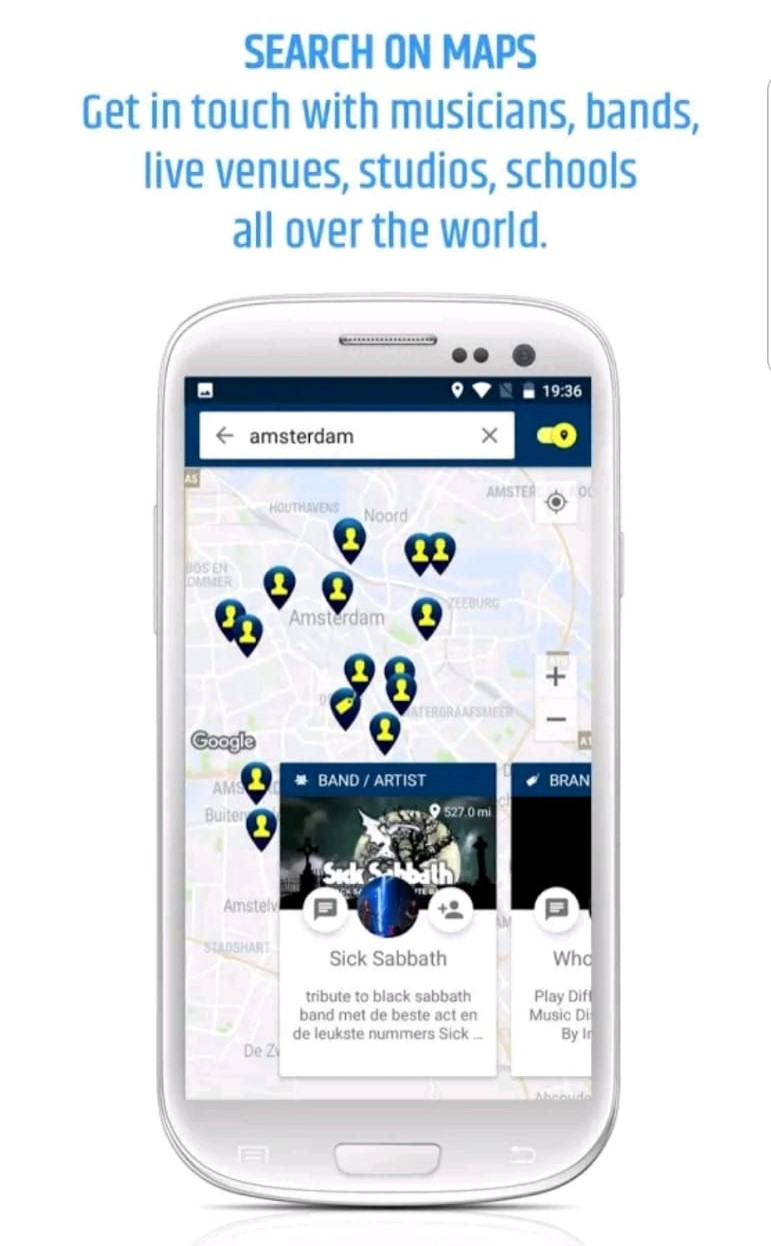
\includegraphics[width=5cm]{slike/Amy.JPEG}
			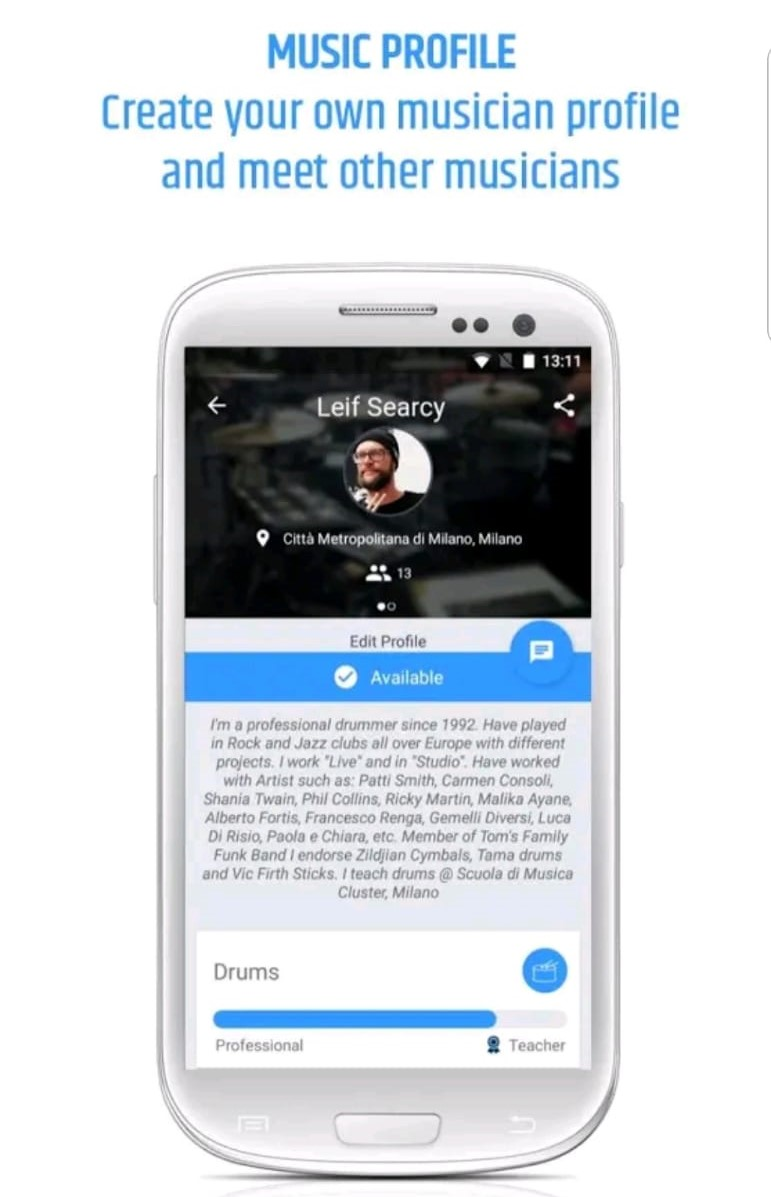
\includegraphics[width=5cm]{slike/Amy2.JPEG}
			\end{center}
			\caption{Izgled \textit{Amy} aplikacije}
			\label{fig:promjene2}
		\end{figure}
		
		
		
	    \subsection{BandFriend}
		
		\textit{BandFriend} je mobilna aplikacija koja prilikom registracije traži dosta informacija o korisniku. Nakon izrade profila, mogu se pretraživati novi glazbenici, glazbenici najsličniji trenutnom korisniku, najbliži po lokaciji i slično. Aplikacija nudi i razgovor porukama s drugim korisnicima. Neke korisnike tolika lista zahtjeva prilikom registracije može odbiti te će \textit{Giger} tražiti samo korisničko ime i lozinku, a kasnije svaki korisnik, ukoliko to želi, može dodati više informacija o sebi. Također, \textit{BandFriend} ne nudi kalendar s obavezama korisnika, stvaranje bendova ili događaja.
		\\
		
		\begin{figure}[H]
			\begin{center}
				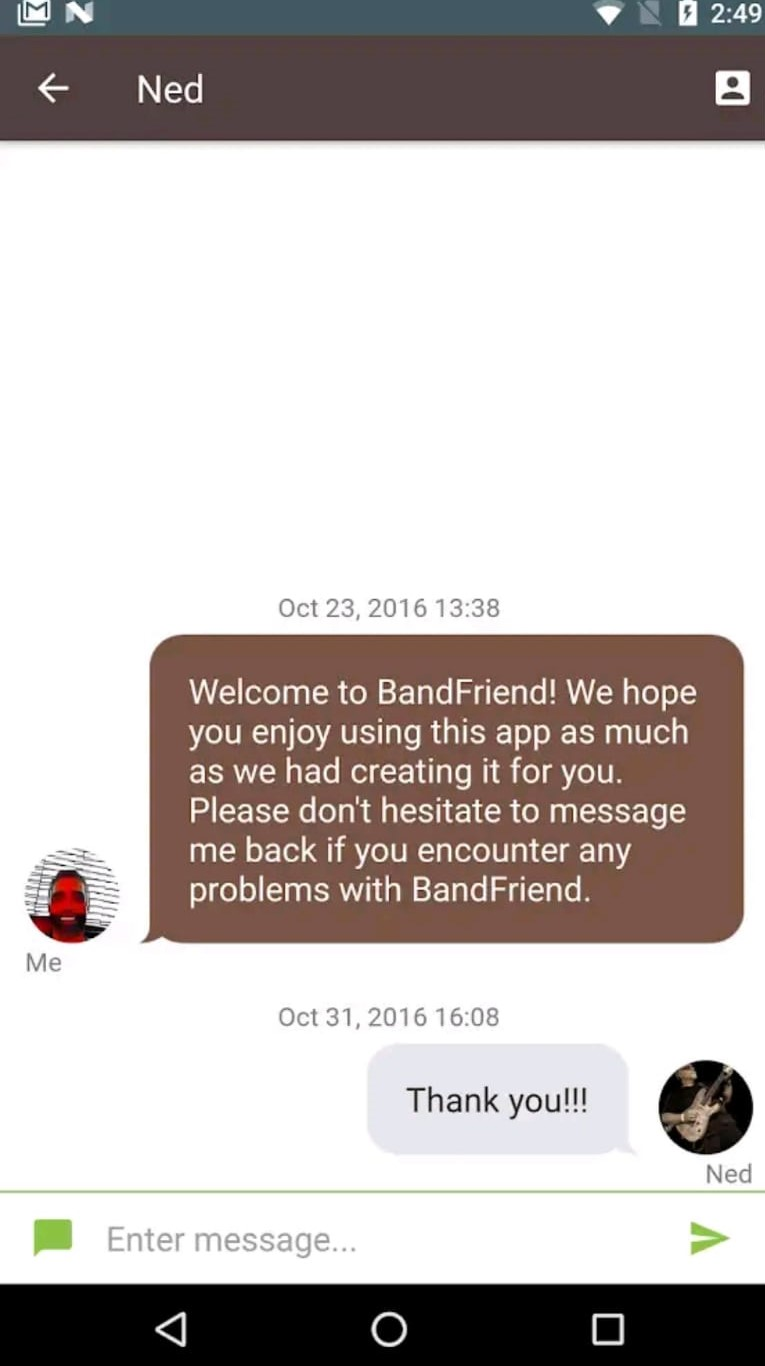
\includegraphics[height=10cm]{slike/BandFriend.JPEG}
				
\includegraphics[height=10cm]{slike/BandFriend2.JPEG}
			\end{center}
			\caption{Izgled \textit{BandFriend} aplikacije}
			\label{fig:promjene3}
		\end{figure}
		 
		
		\section{Primjeri u LaTeXu}
		
		\textit{Ovo potpoglavlje izbrisati.}\\

		U nastavku se nalaze različiti primjeri kako koristiti osnovne funkcionalnosti LaTeXa koje su potrebne za izradu dokumentacije. Za dodatnu pomoć obratiti se asistentu na projektu ili potražiti upute na sljedećim web sjedištima:
		\begin{itemize}
			\item Upute za izradu diplomskog rada u LaTeXu - \url{https://www.fer.unizg.hr/_download/repository/LaTeX-upute.pdf}
			\item LaTeX projekt - \url{https://www.latex-project.org/help/}
			\item StackExchange za Tex - \url{https://tex.stackexchange.com/}\\
		
		\end{itemize} 	


		
		%Ovo poglavlje je potrebno prilikom predaje obrisati
		
		\underbar{podcrtani tekst}, 
		\textbf{podebljani tekst}, 
		\textit{nagnuti tekst}\\
		\normalsize primjer
		\large primjer
		\Large primjer
		\LARGE {primjer}
		\huge {primjer}
		\Huge primjer
		\normalsize
				
		\begin{packed_item}
			
			\item  primjer
			\item  primjer
			\item  primjer
			\item[] \begin{packed_enum}
				
				\item primjer
				\item primjer
			\end{packed_enum}
			
		\end{packed_item}
		
		\noindent primjer url-a: \url{https://www.fer.unizg.hr/predmet/opp/projekt}
		
		
		\begin{longtabu} to \textwidth {|X[8, l]|X[8, l]|X[16, l]|} %definicija sirine polja
			
			\hline \multicolumn{3}{|c|}{\textbf{naslov unutar tablice}}	 \\[3pt] \hline
			\endfirsthead
			
			\hline \multicolumn{3}{|c|}{\textbf{naslov unutar tablice}}	 \\[3pt] \hline
			\endhead
			
			\hline 
			\endlastfoot
			
			\rowcolor{LightGreen}IDKorisnik & INT	&  	Lorem ipsum dolor sit amet, consectetur adipiscing elit, sed do eiusmod  	\\ \hline
			korisnickoIme	& VARCHAR &   	\\ \hline 
			email & VARCHAR &   \\ \hline 
			ime & VARCHAR	&  		\\ \hline 
			\cellcolor{LightBlue} primjer	& VARCHAR &   	\\ \hline 
			
			
		\end{longtabu}
		

		\begin{table}[H]
			
			
			
			\begin{longtabu} to \textwidth {|X[8, l]|X[8, l]|X[16, l]|} %definicija sirine polja
				
				\hline 
				\endfirsthead
				
				\hline 
				\endhead
				
				\hline 
				\endlastfoot
				
				\rowcolor{LightGreen}IDKorisnik & INT	&  	Lorem ipsum dolor sit amet, consectetur adipiscing elit, sed do eiusmod  	\\ \hline
				korisnickoIme	& VARCHAR &   	\\ \hline 
				email & VARCHAR &   \\ \hline 
				ime & VARCHAR	&  		\\ \hline 
				\cellcolor{LightBlue} primjer	& VARCHAR &   	\\ \hline 
				
				
			\end{longtabu}
	
			\caption{\label{tab:referencatablica} Naslov ispod tablice.}
		\end{table}
		
		\begin{figure}[H]
			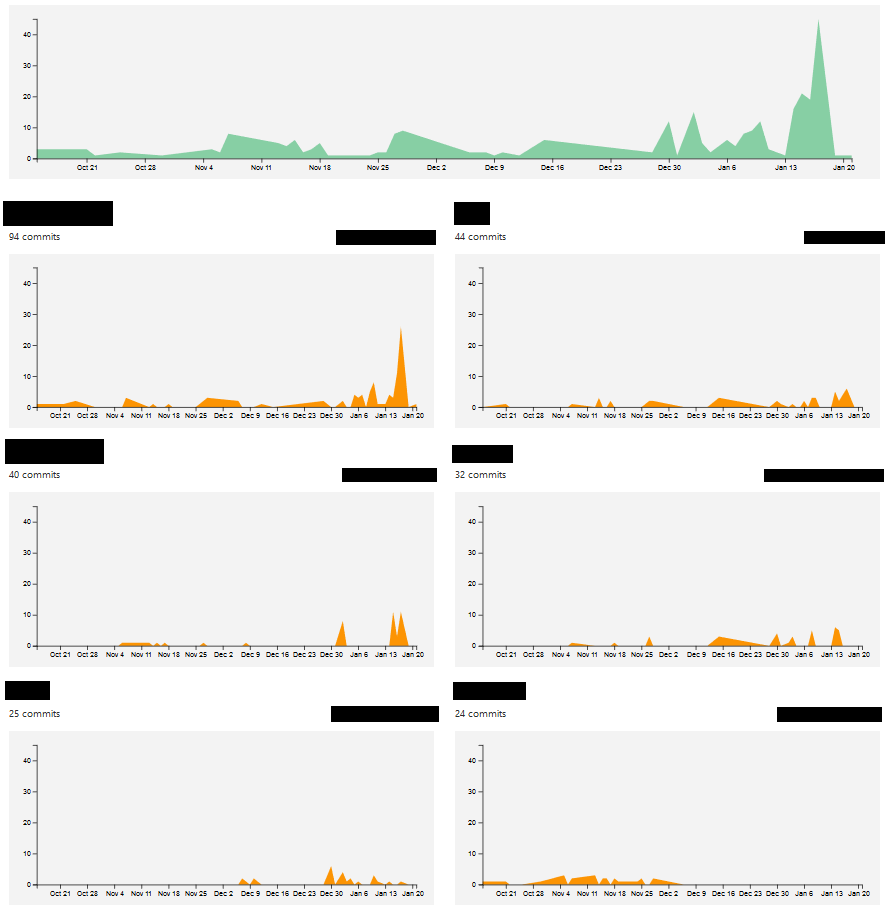
\includegraphics[scale=0.4]{slike/aktivnost.PNG}
			\centering
			\caption{Primjer slike s potpisom}
			\label{fig:promjene}
		\end{figure}
		
		\begin{figure}[H]
			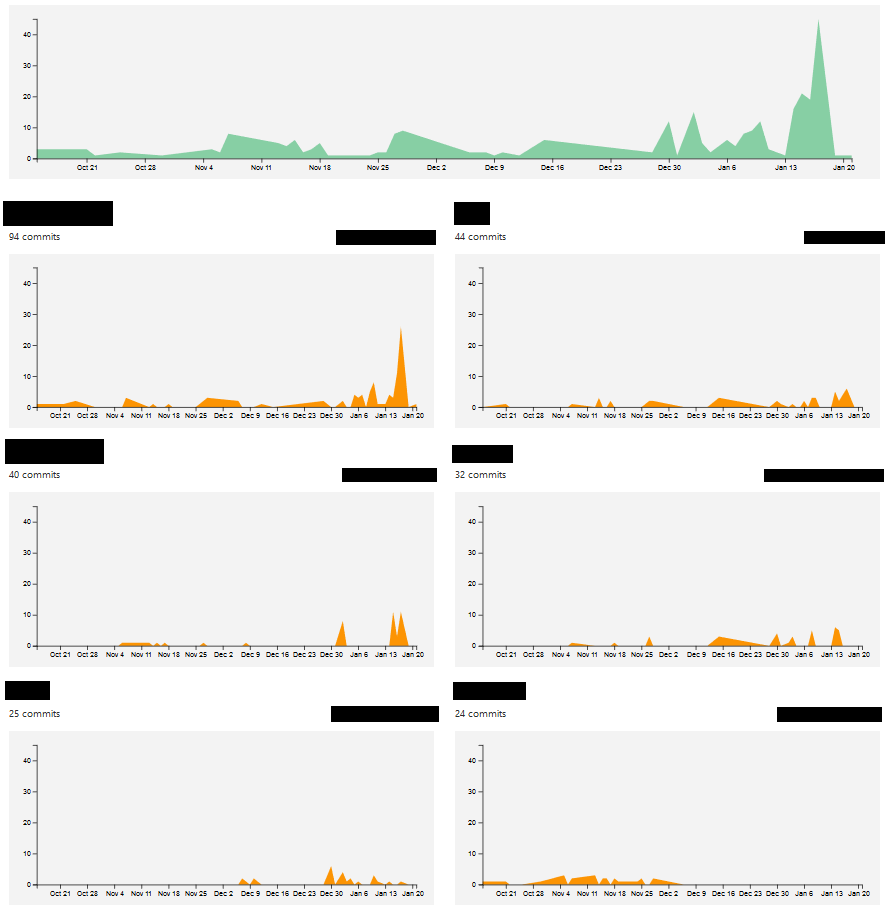
\includegraphics[width=\linewidth]{slike/aktivnost.PNG}
			\caption{Primjer slike s potpisom 2}
			\label{fig:promjen2}
		\end{figure}
		
		
		
		\eject
		
	